\documentclass[11pt]{article}
\usepackage{amsmath,amssymb,amsthm, float}
\usepackage{graphicx} \graphicspath{ {./images/} } % for images
\usepackage[margin=1in]{geometry} % for page dimensions
\usepackage{fancyhdr, enumitem, mathrsfs} % for nice headers, enumerated lists, calligraphic letters
\setlength{\parindent}{0pt}
\setlength{\parskip}{5pt plus 1pt}
\setlength{\headheight}{25.2842pt}
\newcommand\question[2]{\vspace{.25in}\hrule{\textbf{#1}: #2}\vspace{.5em}\hrule\vspace{.10in}}
\renewcommand\part[1]{\vspace{.10in}\textbf{(#1)}}
\newcommand{\todo}{\fbox{TO-DO}\ \ } % for TODOs
% \newcommand\algorithm{\vspace{.10in}\textbf{Algorithm: }}
% \newcommand\correctness{\vspace{.10in}\textbf{Correctness: }}
% \newcommand\runtime{\vspace{.10in}\textbf{Running time: }}
\pagestyle{fancyplain}
\lhead{{\NAME} \\ \EMAILID}
\chead{\textbf{HW \HWNUM}}
\rhead{Capstone: Discrete Math \\ Due: December 14, 2023}
\begin{document}{\raggedright}
%Section A==============Change the values below to match your information==================
\newcommand\NAME{Ojas Chaturvedi}  % your name
\newcommand\EMAILID{oj.chaturvedi.2024@gmail.com}
\newcommand\HWNUM{10} 

\begin{question}
    {5.8.6}
    {
        Let $b_0, b_1, b_2, \ldots$ be the sequence defined by the explicit formula
        \begin{equation*}
            b_n = C \cdot 3^n + D{(-2)}^n \quad \text{for all integers $n \geq 2$}
        \end{equation*}
        where $C$ and $D$ are real numbers. Show that for any choice of $C$ and $D$,
        \begin{equation*}
            b_k = b_{k-1} + 6b_{k-2} \quad \text{for all integers $k \geq 2$}
        \end{equation*}
        \vspace{-\baselineskip}
    }
\end{question}
\begin{proof}
    Let $b_0, b_1, b_2, \ldots$ be the sequence defined by the explicit formula
    \begin{equation*}
        b_n = C \cdot 3^n + D{(-2)}^n \quad \text{for all integers $n \geq 2$}
    \end{equation*}
    We must prove that $b_k$ is true when $b_n$ is plugged in with any choice of $C$ and $D$:
    \begin{align*}
        b_k &= b_{k - 1} + 6b_{k - 2} \\
            &= \left (C\cdot 3^{(k - 1)} + D(-2)^{(k - 1)} \right ) + 6 \left (C\cdot 3^{(k - 2)} + D(-2)^{(k - 2)} \right ) \\
            &= C\cdot 3^{(k - 1)} + D(-2)^{(k - 1)} + 6C\cdot 3^{(k - 2)} + 6D(-2)^{(k - 2)} \\
            &= C \left (3^{(k - 1)} + 2 \left (3^{(k - 1)} \right ) \right ) + D \left ((-2)^{(k - 1)} - 3(-2)^{(k - 1)} \right ) \\
            &= C \left (3 \left (3^{(k - 1)} \right ) \right ) + D \left (-2(-2)^{(k - 1)} \right ) \\
            &= C (3^k) + D(-2)^k \\
            &= b_k
    \end{align*}
    Thus, we have proved that, for any choice of $C$ and $D$,
    \begin{equation*}
        b_k = b_{k-1} + 6b_{k-2} \quad \text{for all integers $k \geq 2$}
    \end{equation*}
    \vspace{-\baselineskip}
\end{proof}

\begin{question}
    {5.8.9}
    {
        \begin{enumerate}
            \item[a.] Suppose a sequence of the form $1,t,t^2,t^3, \ldots, t^n \ldots$ where $t \neq 0$, satisfies the given recurrence relation (but not necessarily the initial conditions), and find all possible values of $t$.
            \item[b.] Suppose a sequence satisfies the given initial conditions as well as the recurrence relation, and find an explicit formula for the sequence.
        \end{enumerate}
        \begin{equation*}
            b_k = 7b_{k-1} - 10b_{k-2} \quad \text{for all integers $k \geq 2$}
        \end{equation*}
        \begin{equation*}
            b_0 = 2 \quad b_1=2
        \end{equation*}
        \vspace{-\baselineskip}
    }
\end{question}
\begin{proof}
    \begin{enumerate}
        \item[a.] 
            Suppose a sequence of the form $1,t,t^2,t^3, \ldots, t^n \ldots$ where $t \neq 0$, satisfies 
            \begin{equation*}
                b_k = 7b_{k-1} - 10b_{k-2} \quad \text{for all integers $k \geq 2$}
            \end{equation*}
            Since we suppose the sequence is of form $1, t, t^2, \ldots, t^n, \ldots$, by the characteristic equation of the second-order linear homogeneous recurrence relation with constant coefficients, 
            \begin{align*}
                t^2 - 7t + 10 &= 0 \\
                (t - 5)(t - 2) &= 0 \\
                t &= 2, 5
            \end{align*}
            Thus, the only possible values of $t$ are $2$ and $5$.
        \item[b.] 
            $b_0, b_1, b_2, \ldots$ satisfies the equation
            \begin{equation*}
                b_n = C\cdot 2^n + D\cdot 5^n \quad \text{for all integers $n \geq 0$}
            \end{equation*}
            for some constants $C$ and $D$ due to part (a) and the distinct roots theorem. We are given that $b_0 = 2, b_1 = 2$. Therefore, 
            \begin{align*}
                &\begin{cases} 
                    b_0 = C \cdot 2^0 + D \cdot 5^0 \\
                    b_1 = C \cdot 2^1 + D \cdot 5^1
                \end{cases}
                &\begin{cases} 
                    2 = C + D \\ 
                    2 = 2C + 5D
                \end{cases}
            \end{align*}
            Plugging in $C = 2 - D$, 
            \begin{align*}
                2(2 - D) + 5D &= 2 \\
                4 - 2D + 5D &= 2 \\
                4 + 3D &= 2 \\
                3D &= -2 \\
                D &= \dfrac{-2}{3}
            \end{align*}
            Thus,
            \begin{equation*}
                b_n = C\cdot 2^n + D\cdot 5^n \quad \text{for all integers $n \geq 0$}
            \end{equation*}
            \vspace{-\baselineskip}
            \begin{align*}
                C &= 2 - D \\
                D &= \dfrac{-2}{3} \\
                C &= \dfrac{8}{3}
            \end{align*}
            \vspace{-\baselineskip}
            \begin{equation*}
                b_n = \dfrac{8}{3}\cdot 2^n + \dfrac{-2}{3}\cdot 5^n \quad \text{for all integers $n \geq 0$}
            \end{equation*}
    \end{enumerate}
\end{proof}

\begin{question}
    {5.8.10}
    {
        \begin{enumerate}
            \item[a.] Suppose a sequence of the form $1,t,t^2,t^3, \ldots, t^n \ldots$ where $t \neq 0$, satisfies the given recurrence relation (but not necessarily the initial conditions), and find all possible values of $t$.
            \item[b.] Suppose a sequence satisfies the given initial conditions as well as the recurrence relation, and find an explicit formula for the sequence.
        \end{enumerate}
        \begin{equation*}
            c_k = c_{k-1} + 6c_{k-2} \quad \text{for all integers $k \geq 2$}
        \end{equation*}
        \begin{equation*}
            c_0 = 0 \quad c_1=3
        \end{equation*}
    }
\end{question}
\begin{proof}
    \begin{enumerate}
        \item[a.] 
            Suppose a sequence of the form $1,t,t^2,t^3, \ldots, t^n \ldots$ where $t \neq 0$, satisfies 
            \begin{equation*}
                c_k = c_{k-1} + 6c_{k-2} \quad \text{for all integers $k \geq 2$}
            \end{equation*}
            Since we suppose the sequence is of form $1, t, t^2, \ldots, t^n, \ldots$, by the characteristic equation of the second-order linear homogeneous recurrence relation with constant coefficients, 
            \begin{align*}
                t^2 - t - 6 &= 0 \\
                (t - 3)(t + 2) &= 0 \\
                t &= -2, 3
            \end{align*}
            Thus, the only possible values of $t$ are $-2$ and $3$.
        \item[b.] 
            $c_0, c_1, c_2, \ldots$ satisfies the equation
            \begin{equation*}
                c_n = C\cdot (-2)^n + D\cdot 3^n \quad \text{for all integers $n \geq 0$}
            \end{equation*}
            for some constants $C$ and $D$ due to part (a) and the distinct roots theorem. We are given that $c_0 = 0, c_1 = 3$. Therefore, 
            \begin{align*}
                &\begin{cases} 
                    c_0 = C\cdot (-2)^0 + D\cdot 3^0 \\
                    c_1 = C\cdot (-2)^1 + D\cdot 3^1
                \end{cases}
                &\begin{cases} 
                    0 = C + D \\
                    3 = -2C + 3D
                \end{cases}
            \end{align*}
            Plugging in $C = - D$, 
            \begin{align*}
                -2(-D) + 3D &= 3 \\
                2D + 3D &= 3 \\
                5D &= 3 \\
                D &= \dfrac{3}{5}
            \end{align*}
            Thus,
            \begin{equation*}
                c_n = C\cdot (-2)^n + D\cdot 3^n \quad \text{for all integers $n \geq 0$}
            \end{equation*}
            \vspace{-\baselineskip}
            \begin{align*}
                C &= - D \\
                D &= \dfrac{3}{5} \\
                C &= \dfrac{-3}{5}
            \end{align*}
            \vspace{-\baselineskip}
            \begin{equation*}
                c_n = \dfrac{-3}{5}\cdot (-2)^n + \dfrac{3}{5}\cdot 3^n \quad \text{for all integers $n \geq 0$}
            \end{equation*}
    \end{enumerate}
\end{proof}

\begin{question}
    {5.8.15}
    {
        Suppose a sequence satisfies the given recurrence relation and initial conditions. Find an explicit formula for the sequence.
        \begin{equation*}
            t_k = 6t_{k-1} - 9t_{k-2} \quad \text{for all integers $k \geq 2$}
        \end{equation*}
        \begin{equation*}
            t_0 = 1 \quad t_1=3
        \end{equation*}
    }
\end{question}
\begin{proof}
    Suppose a sequence of the form $t_0, t_1, t_2, \ldots$ satisfies 
    \begin{equation*}
        t_k = 6t_{k-1} - 9t_{k-2} \quad \text{for all integers $k \geq 2$}
    \end{equation*}
    Since we suppose the sequence is of form $t_0, t_1, t_2, \ldots$, by the characteristic equation of the second-order linear homogeneous recurrence relation with constant coefficients,
    \begin{align*}
        y^2 &- 6a + 9 = 0 \\
        y &= 3
    \end{align*}
    for some number $y$ that satisfies the Characteristic Equation. 
    Thus, the only possible value of $y$ is 3.
    Due to the single-root theorem, $t_0, t_1, t_2, \ldots$ satisfies the equation
    \begin{equation*}
        t_n = Cr^n + Dnr^n \quad \text{for all integers $n \geq 0$}
    \end{equation*}
    for some constants $C$ and $D$ and real root $r$.
    % Since $t_0 = 1, t_1 = 3$, then
    We are given that $t_0 = 1, t_1 = 3$. Therefore,
    \begin{align*}
        &\begin{cases}
            t_0 = C\cdot 3^0 + D(0)\cdot 3^0 \\
            c_1 = C\cdot 3^1 + D\cdot 3^1
        \end{cases}
        &\begin{cases} 
            1 = C \\ 
            3 = 3C + 3D
        \end{cases}
        &\begin{cases} 
            C = 1 \\ 
            D = 0
        \end{cases}
    \end{align*}
    Hence,
    \begin{equation*}
        t_n = 3^n \quad \text{for all integers $n \geq 0$}
    \end{equation*}
\end{proof}

\newpage
\begin{question}
    {5.8.24}
    {
        The numbers $\dfrac{1 + \sqrt{5}}{2}$ and $\dfrac{1 - \sqrt{5}}{2}$ that appear in the explicit formula for the Fibonacci sequence are related to a quantity called the \textit{golden ration} in Greek mathematics. Consider a rectangle of length $\phi$ units and height $1$, where $\phi > 1$.
        \begin{figure}[H]
            \centering
            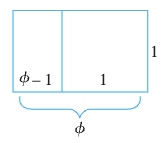
\includegraphics{5.8.24}
        \end{figure}
        Divide the rectangle into a rectangle and a square as shown in the preceding diagram. The square is $1$ unit on each side, and the rectangle has sides of length $1$ and $\phi - 1$.
        The ancient Greeks considered the outer rectangle to be perfectly proportioned (saying that the lengths of its sides were in a \textit{golden ratio} to each other) if the ratio of the length to the width of the outer rectangle equaled the ratio of the length to the width of the inner rectangle. That is,
        \begin{equation*}
            \frac{\phi}{1} = \frac{1}{\phi - 1}
        \end{equation*}
        \begin{enumerate}
            \item[a.] Show that $\phi$ satisfies the following quadratic equation $t^2 - t - 1 = 0$.
            \item[b.] Find the two solutions of $t^2 - t - 1 = 0$ and call them $\phi_1$ and $\phi_2$.
            \item[c.] Express the explicit formula for the Fibonacci sequence in terms of $\phi_1$ and $\phi_2$.
        \end{enumerate}
    }
\end{question}
\begin{proof}
    \begin{enumerate}
        \item[a.]
        \begin{align*}
            \frac{\phi}{1} &= \frac{1}{\phi - 1} \\
            \phi \cdot (\phi - 1) &= 1 \\
            \phi^2 - \phi &= 1 \\
            \phi^2 - \phi - 1 &= 0
        \end{align*}
        which is in the form $t^2 - t - 1 = 0$. Hence, $\phi$ satisfies the quadratic equation $t^2 - t - 1 = 0$.
        \item[b.]
        \begin{align*}
            \phi_1, \phi_2 &= \frac{-b \pm \sqrt{b^2 - 4ac}}{2a} \\
            &= \frac{1 \pm \sqrt{1 + 4}}{2} \\
            &= \frac{1 + \sqrt{1 + 4}}{2}, \frac{1 - \sqrt{1 + 4}}{2} \\
            &= \frac{1 + \sqrt{5}}{2}, \frac{1 - \sqrt{5}}{2} \\
            \phi_1 &= \frac{1 + \sqrt{5}}{2} \\
            \phi_2 &= \frac{1 - \sqrt{5}}{2}
        \end{align*}
        \item[c.] We know that the characteristic equation of the Fibonacci sequence has the solutions $\phi_1, \phi_2$. Due to the distinct-roots theorem, the Fibonacci sequence is given by the explicit formula:
        \begin{equation*}
            F_n = C\phi_1^n + D\phi_2^n \quad \text{for all integers $n \geq 0$}
        \end{equation*}
        for some constants $C$ and $D$. We are given that $F_0 = 0, F_1 = 1$. Therefore, when substituting for $n = 0, 1$ \\
        \begin{align*}
            \begin{cases}
                C + D = 1 \\ C\phi_1 + D\phi_2 = 1
            \end{cases}
        \end{align*}
        Plugging in $C = 1 - D$,
        \begin{align*}
            (1 - D)\phi_1 + D\phi_2 &= 1 \\
            D(\phi_2 - \phi_1) &= 1 - \phi_1 \\
            D &= \frac{1 - \phi_1}{\phi_2 - \phi_1}
        \end{align*}
        Thus,
        \begin{align*}
            C &= 1 - D \\
            C &= 1 - \frac{1 - \phi_1}{\phi_2 - \phi_1} \\
            C &= \frac{\phi_2 - \phi_1}{\phi_2 - \phi_1} - \frac{1 - \phi_1}{\phi_2 - \phi_1} \\
            C &= \frac{\phi_2 - 1}{\phi_2 - \phi_1}
        \end{align*}
        Therefore, the explicit formula for the Fibonacci Sequence in terms of $\phi_1$ and $\phi_2$ can be written as
        \begin{equation*}
            F_n = \dfrac{\phi_2 - 1}{\phi_2 - \phi_1}(\phi_1^n) + \dfrac{1 - \phi_1}{\phi_2 - \phi_1}(\phi_2^n) \quad \text{for all integers $n \geq 0$}
        \end{equation*}
    \end{enumerate}
\end{proof}
\begin{question}
    {5.9.4b}
    {
        The set of arithmetic expressions over the real numbers can be defined recursively as follows:
        \vspace{-\baselineskip}
        \begin{enumerate}[label=\Roman*.]
            \item BASE:\@ Each real number $r$ is an arithmetic expression.
            \item RECURSION:\@ If $u$ and $v$ are arithmetic expressions, then the following are also arithmetic expressions:
                \begin{enumerate}
                    \item[a.] ($+u$)
                    \item[b.] ($-u$)
                    \item[c.] ($u + v$)
                    \item[d.] ($u - v$)
                    \item[e.] ($u \cdot v$)
                    \item[f.] $\left(\dfrac{u}{v} \right)$
                \end{enumerate}
            \item RESTRICTION:\@ There are no arithmetic expressions over the real numbers other than those obtained from I and II.\@
        \end{enumerate}
        \vspace{-\baselineskip}
        (Note that the \textit{expression} $\left(\dfrac{u}{v} \right)$ is legal even though the value of $v$ may be $0$.) Give derivations showing that each of the following is an arithmetic expression.
        \begin{align*}
            \left(\dfrac{(9 \cdot (6.1 + 2))}{((4-7) \cdot 6)} \right)
        \end{align*}
    }
\end{question}
\begin{proof}
    \begin{enumerate}
        \item According to BASE (I), numbers 9, 6.1, 2, 4, 7, and 6 are each arithmetic expressions.
        \item Utilizing (1) and RECURSION II(c), the expression \(6.1 + 2\) qualifies as an arithmetic expression.
        \item From (1), (2), and RECURSION II(e), the expression \(9 \cdot (6.1 + 2)\) is an arithmetic expression.
        \item Using (1) and RECURSION II(d), the expression \(4 - 7\) is an arithmetic expression.
        \item Applying (1), (4), and RECURSION II(e), the expression \((4 - 7) \cdot 6\) is an arithmetic expression.
        \item Combining (3), (5), and RECURSION II(f), the expression \(\dfrac{9 \cdot (6.1 + 2)}{(4 - 7) \cdot 6}\) is confirmed to be an arithmetic expression.
    \end{enumerate}
    \vspace{-\baselineskip}
\end{proof}

\begin{question}
    {5.9.6}
    {
        Define a set $S$ recursively as follows:
        \vspace{-\baselineskip}
        \begin{enumerate}[label=\Roman*.]
            \item BASE:\@ $a \in S$
            \item RECURSION:\@ If $s \in S$, then
                \begin{enumerate}
                    \item[a.] $sa \in S$
                    \item[b.] $sb \in S$
                \end{enumerate}
            \item RESTRICTION:\@ Nothing is in $S$ other than objects defined in I and II above.
        \end{enumerate}
        \vspace{-\baselineskip}
        Use structural induction to prove that every string in $S$ begins with an $a$.
    }
\end{question}
\begin{proof}
    The proof is conducted using structural induction to demonstrate that every string in \(S\) begins with an 'a'. \\ \\
    \textbf{\textit{Base Case:}} \\
    The base case involves the string 'a', as defined by BASE (I). Clearly, 'a' begins with an 'a', satisfying the property. \\ \\
    \textbf{\textit{Inductive Step:}} \\
    Assume for the recursion step that any string \(s \in S\) begins with 'a', a hypothesis based on the RECURSION rule (II). According to rules II(a) and II(b), if \(s \in S\), then both 'sa' and 'sb' are in \(S\). Given our hypothesis, 'sa' and 'sb' also begin with 'a'.  \\ \\
    \textbf{\textit{Conclusion:}} \\
    Since both the base case and the inductive step hold, and no elements are in \(S\) other than those defined in BASE and RECURSION, we conclude that every string in \(S\) begins with an 'a'.
\end{proof}

\begin{question}
    {5.9.11}
    {
        Define a set $S$ recursively as follows:
        \vspace{-\baselineskip}
        \begin{enumerate}[label=\Roman*.]
            \item BASE:\@ $0 \in S$
            \item RECURSION:\@ If $s \in S$, then
                \begin{enumerate}
                    \item[a.] $s + 3 \in S$
                    \item[b.] $s - 3 \in S$
                \end{enumerate}
            \item RESTRICTION:\@ Nothing is in $S$ other than objects defined in I and II above.
        \end{enumerate}
        \vspace{-\baselineskip}
        Use structural induction to prove that every integer in $S$ is divisible by $3$.
    }
\end{question}
\begin{proof}
    The proof employs structural induction to establish that every integer in \(S\) is divisible by 3. \\ \\
    \textbf{\textit{Base Case:}} \\
    The BASE (I) of \(S\) includes the integer 0. Since 0 is divisible by 3, it fulfills the property. \\ \\
    \textbf{\textit{Inductive Step:}} \\
    For the inductive step, assume that any integer \(s \in S\) is divisible by 3. This is based on the RECURSION rule (II). According to rules II(a) and II(b), if \(s \in S\), then \(s + 3\) and \(s - 3\) also belong to \(S\). If \(s\) is divisible by 3, it can be represented as \(s = 3k\) for some integer \(k\). Therefore, both \(s + 3\) and \(s - 3\) are divisible by 3, as they can be expressed as \(3(k + 1)\) and \(3(k - 1)\), respectively. \\ \\
    \textbf{\textit{Conclusion:}} \\
    Given that the base case is satisfied and the inductive step holds, and considering that no elements other than those derived through BASE and RECURSION are in \(S\), it can be concluded that every integer in \(S\) is divisible by 3.
\end{proof}

\begin{question}
    {5.9.16}
    {
        Give a recursive definition for the set of all strings of $0$'s and $1$'s for which all the $0$'s precede all the $1$'s.
    }
\end{question}
\begin{proof}
    Let $S$ be the set of all strings of 0's and 1's for which all the 0's precede all the 1's. Here is the recursive definition for $S$:
    \begin{enumerate}
        \item[\textbf{I.}] BASE: $\epsilon \in S$
        \item[\textbf{II.}] RECURSION: If $s \in S$, then $0s \in S$ and $s1 \in S$
        \item[\textbf{III.}] RESTRICTION: There are no elements of $S$ other than those inferred from rules I and II.
    \end{enumerate}
    \vspace{-\baselineskip}
\end{proof}

\begin{question}
    {5.9.18}
    {
        Give a recursive definition for the set of all strings of $a$'s and $b$'s that contain exactly one $a$.
    }
\end{question}
\begin{proof}
    Let $S$ be the set of all strings of $a$'s and $b$'s that contain exactly one $a$. The following is a recursive definition of $S$:
    \begin{enumerate}
        \item[\textbf{I.}] BASE: $a \in S$
        \item[\textbf{II.}] RECURSION: If $s \in S$, then $sb \in S$ and $bs \in S$
        \item[\textbf{III.}] RESTRICTION: There are no elements of $S$ other than those inferred from rules I and II.
    \end{enumerate}
    \vspace{-\baselineskip}
\end{proof}
\begin{question}
    {6.1.6}
    {
        Let $A=\{x \in \mathbf{Z} \mid x=5 a+2$ for some integer $a\}$, $B=\{y \in \mathbf{Z} \mid y=10 b-3$ for some integer $b\}$, and $C=\{z \in \mathbf{Z} \mid z=10 c+7$ for some integer $c\}$. Prove or disprove each of the following statements.
        \vspace{-\baselineskip}
        \begin{enumerate}
            \item[a.] $A \subseteq B$
            \item[b.] $B \subseteq A$
            \item[c.] $B=C$
        \end{enumerate}
    }
\end{question}
\begin{proof}
    Let $A=\{x \in \mathbf{Z} \mid x=5 a+2$ for some integer $a\}$, $B=\{y \in \mathbf{Z} \mid y=10 b-3$ for some integer $b\}$, and $C=\{z \in \mathbf{Z} \mid z=10 c+7$ for some integer $c\}$. 
    \begin{enumerate}
        \item[a.] Disprove $A \subseteq B$ using a counterexample: \\
        Consider $x = 2 \in A$ for $a = 0$. For $x$ to be in $B$, we need $10b - 3 = 2$, leading to $b = 0.5$, a contradiction since $b$ must be an integer. Therefore, $A \not\subseteq B$.
        \item[b.] 
        Let $x \in B$, so $x = 10b - 3$ for some integer $b$. Then $x = 5(2b - 1) + 2$, which means there exists an integer $a = 2b - 1$ such that $x \in A$. Therefore, $B \subseteq A$.
        \item[c.] 
        To show $B \subseteq C$, let $x \in B$. Then $x = 10b - 3$ and setting $c = b - 1$, we get $x = 10c + 7$, thus $x \in C$. To show $C \subseteq B$, let $x \in C$. Then $x = 10c + 7$ and setting $b = c + 1$, we get $x = 10b - 3$, thus $x \in B$. Hence, $B = C$.
    \end{enumerate}
    \vspace{-\baselineskip}
\end{proof}

\begin{question}
    {6.1.20}
    {
        Let $B_i=\{x \in \mathbf{R} \mid 0 \leq x \leq i\}$ for all integers $i=1,2,3,4$.
        \vspace{-\baselineskip}
        \begin{enumerate}
            \item[a.] $B_1 \cup B_2 \cup B_3 \cup B_4=$ ?
            \item[b.] $B_1 \cap B_2 \cap B_3 \cap B_4=$ ?
            \item[c.] Are $B_1, B_2, B_3$, and $B_4$ mutually disjoint? Explain.
        \end{enumerate}
    }
\end{question}
\begin{proof}
    \begin{enumerate}
        \item[a.] $\{x \in \mathbf{R} \mid 0 \leq x \leq 4\}$
        \item[b.] $\{x \in \mathbf{R} \mid 0 \leq x \leq 1\}$
        \item[c.] The sets $B_1, B_2, B_3$, and $B_4$ are not mutually disjoint. For instance, the number 1 is included in all these sets. More generally, if a number is in $B_i$, it will be in all $B_j$ for $j \geq i$.
    \end{enumerate}
    \vspace{-\baselineskip}
\end{proof}

\begin{question}
    {6.1.23}
    {
        Let $V_i=\left\{x \in \mathbf{R} \mid-\dfrac{1}{i} \leq x \leq \dfrac{1}{i}\right\}=\left[-\dfrac{1}{i}, \dfrac{1}{i}\right]$ for all positive integers $i$.
        \vspace{-\baselineskip}
        \begin{enumerate}
            \item[a.] $\bigcup_{i=1}^4 V_i=$ ?
            \item[b.] $\bigcap_{i=1}^4 V_i=$ ?
            \item[c.] Are $V_1, V_2, V_3, \ldots$ mutually disjoint? Explain.
            \item[d.] $\bigcup_{i=1}^n V_i=$ ?
            \item[e.] $\bigcap_{i=1}^n V_i=$ ?
            \item[f.] $\bigcup_{i=1}^{\infty} V_i=$ ?
            \item[g.] $\bigcap_{i=1}^{\infty} V_i=$ ?
        \end{enumerate}
    }
\end{question}
\begin{proof}
    \begin{enumerate}
        \item[a.] $\bigcup_{i=1}^4 V_i = [-1, 1]$
        \item[b.] $\bigcap_{i=1}^4 V_i = \left[-\frac{1}{4}, \frac{1}{4}\right]$
        \item[c.] The sets $V_1, V_2, V_3, \ldots$ are not mutually disjoint since they all contain the point 0.
        \item[d.] $\bigcup_{i=1}^n V_i = [-1, 1]$ for any positive integer $n$.
        \item[e.] $\bigcap_{i=1}^n V_i = \{0\}$ as $n \rightarrow \infty$.
        \item[f.] $\bigcup_{i=1}^{\infty} V_i = [-1, 1]$
        \item[g.] $\bigcap_{i=1}^{\infty} V_i = \{0\}$
    \end{enumerate}    
\end{proof}

\begin{question}
    {6.1.33}
    {
        \vspace{-\baselineskip}
        \begin{enumerate}
            \item[a.] Find $\mathscr{P}(\emptyset)$.
            \item[b.] Find $\mathscr{P}(\mathscr{P}(\emptyset))$.
            \item[c.] Find $\mathscr{P}(\mathscr{P}(\mathscr{P}(\emptyset)))$.
        \end{enumerate}
    }
\end{question}
\begin{proof}
    \begin{enumerate}
        \item[a.] 
        \begin{equation*}
            \mathscr{P}(\emptyset) = \{\emptyset\}
        \end{equation*}
    
        \item[b.] 
        \begin{equation*}
            \mathscr{P}(\mathscr{P}(\emptyset)) = \{\emptyset, \{\emptyset\}\}
        \end{equation*}
    
        \item[c.] 
        \begin{equation*}
            \mathscr{P}(\mathscr{P}(\mathscr{P}(\emptyset))) = \{\emptyset, \{\emptyset\}, \{\{\emptyset\}\}, \{\emptyset, \{\emptyset\}\}\}
        \end{equation*}
    \end{enumerate}
\end{proof}

\begin{question}
    {6.2.10}
    {
        Use an element argument to prove the statement.
        Assume that all sets are subsets of a universal set $U$.
        For all sets $A, B$, and $C$,
        \begin{align*}
            (A-B) \cap(C-B)=(A \cap C)-B \text{. }
        \end{align*}
        \vspace{-\baselineskip}
    }
\end{question}
\begin{proof}
    Consider arbitrary sets \(A, B, C\). The given statement is proven true by establishing two key sub-statements:
    \begin{enumerate}
        \item[1.] \((A - B) \cap (C - B) \subseteq (A \cap C) - B\)
        \item[2.] \((A \cap C) - B \subseteq (A - B) \cap (C - B)\)
    \end{enumerate}
    Firstly, for statement 1: \\
    Let \(x\) be an element of \((A - B) \cap (C - B)\). \\
    Since \(x\) is in the intersection, it must be in both \(A - B\) and \(C - B\). Thus, \(x\) belongs to \(A\) and \(C\) but not to \(B\). Consequently, \(x\) is an element of \(A \cap C\) and not in \(B\), leading to \(x\) being in \((A \cap C) - B\). This confirms \((A - B) \cap (C - B) \subseteq (A \cap C) - B\). \\ \\
    Next, for statement 2: \\
    Take \(x\) as an element of \((A \cap C) - B\). \\
    From the set difference and intersection definitions, \(x\) is in both \(A\) and \(C\), and not in \(B\). Hence, \(x\) lies in both \(A - B\) and \(C - B\). Therefore, by intersection properties, \(x\) is in \((A - B) \cap (C - B)\). \\
    This confirms \((A \cap C) - B \subseteq (A - B) \cap (C - B)\).
    Since both sub-statements are proven, it follows that \((A - B) \cap (C - B) = (A \cap C) - B\), thereby validating the original statement.
\end{proof}

\begin{question}
    {6.2.14}
    {
        Use an element argument to prove the statement.
        Assume that all sets are subsets of a universal set $U$.
        For all sets $A, B$, and $C$, if $A \subseteq B$ then $A \cup C \subseteq B \cup C$.
    }
\end{question}
\begin{proof}
    Assume sets \(A, B, C\) with \(A \subseteq B\). Consider an arbitrary element \(x\). Assume \(x \in A \cup C\). According to the definition of union, this implies \(x \in A\) or \(x \in C\). \\ \\
    \textbf{\textit{Case 1:}} \(x \in A\): \\
    Given \(A \subseteq B\), if \(x\) is in \(A\), it must also be in \(B\). Hence, by the nature of union, \(x\) is in \(B \cup C\). \\ \\
    \textbf{\textit{Case 2:}} \(x \in C\): \\
    Directly by the definition of union, if \(x\) is in \(C\), it is necessarily in \(B \cup C\).
    In both scenarios, \(x \in B \cup C\) is validated. Thus, it is concluded that \(A \cup C \subseteq B \cup C\).
\end{proof}

\begin{question}
    {6.2.32}
    {
        Use the element method for proving a set equals the empty set to prove the statement.
        Assume that all sets are subsets of a universal set $U$.
        For all sets $A, B$, and $C$, if $A \subseteq B$ and $B \cap C=\emptyset$ then $A \cap C=\emptyset$.
    }
\end{question}
\begin{proof}
    To prove the statement, assume the contrary. Consider sets \(A, B, C\) such that \(A \subseteq B\) and \(B \cap C = \emptyset\). The negation of the statement is \(A \cap C \neq \emptyset\), implying the existence of an element \(x\) such that \(x \in A\) and \(x \in C\). \\ \\
    Since \(x \in A\) and \(A \subseteq B\), it follows that \(x \in B\). However, if \(x \in C\) and \(B \cap C = \emptyset\), this leads to a contradiction because \(x\) cannot be in both \(B\) and \(C\) if their intersection is empty. \\ \\
    This contradiction disproves the negation, thereby proving the original statement: If \(A \subseteq B\) and \(B \cap C = \emptyset\), then \(A \cap C = \emptyset\).
\end{proof}

\begin{question}
    {6.2.39}
    {
        Prove the statement.
        For all integers $n \geq 1$, if $A_1, A_2, A_3, \ldots$ and $B$ are any sets, then
        \begin{align*}
            \bigcap_{i=1}^n (A_i - B) = \left(\bigcap_{i=1}^n A_i \right) - B \text{. }
        \end{align*}
    }
\end{question}
\begin{proof}
    Assume \(A_1, A_2, A_3, \ldots\) and \(B\) are arbitrary sets. The statement is proven by showing:
    \begin{enumerate}
        \item[1.] \(\left[\bigcap_{i = 1}^n (A_i - B)\right] \subseteq \left[\bigcap_{i = 1}^n A_i\right] - B\)
        \item[2.] \(\left[\bigcap_{i = 1}^n A_i\right] - B \subseteq \left[\bigcap_{i = 1}^n (A_i - B)\right]\)
    \end{enumerate}
    First, to prove statement 1: \\
    Let \(x\) be an element of \(\bigcap_{i = 1}^n (A_i - B)\). This means \(x\) is in each \(A_i - B\) for all \(i\), so \(x\) is in every \(A_i\) and not in \(B\). Therefore, \(x\) is in \(\bigcap_{i = 1}^n A_i\) and, by set difference, \(x\) is in \(\left(\bigcap_{i = 1}^n A_i\right) - B\). \\ \\
    Next, to prove statement 2: \\
    Consider \(x\) as an element of \((\bigcap_{i = 1}^n A_i) - B\). By set difference, \(x\) is in \(\bigcap_{i = 1}^n A_i\) and not in \(B\). Hence, \(x\) is in each \(A_i\) and not in \(B\), implying \(x\) is in every \(A_i - B\), and therefore in \(\bigcap_{i = 1}^n (A_i - B)\). \\ \\
    As both sub-statements are confirmed, it follows that \(\bigcap_{i = 1}^n (A_i - B) = \left(\bigcap_{i = 1}^n A_i\right) - B\), thus proving the original statement.
\end{proof}

\end{document}